El sistema implementa perfiles de velocidad trapezoidales para garantizar movimientos suaves, minimizando vibraciones mecánicas y errores de posicionamiento por pérdida de pasos.

\subsubsection{Perfil Trapezoidal de Velocidad}

El perfil trapezoidal divide cada movimiento en 5 zonas con transiciones graduales (Figura \ref{fig:perfil_trapezoidal}):

\begin{enumerate}
    \item \textbf{Aceleración suave} (15\% del recorrido): Rampa lineal desde velocidad inicial (500 pasos/s) hasta velocidad baja (2000 pasos/s)
    \item \textbf{Aceleración fuerte} (10\% del recorrido): Rampa lineal desde velocidad baja hasta velocidad crucero (hasta 15,000 pasos/s para eje horizontal, 12,000 pasos/s para eje vertical)
    \item \textbf{Crucero} (50\% del recorrido): Velocidad constante máxima, minimizando vibraciones
    \item \textbf{Desaceleración fuerte} (10\% del recorrido): Rampa lineal desde velocidad crucero hasta velocidad baja
    \item \textbf{Desaceleración suave} (15\% del recorrido): Rampa lineal desde velocidad baja hasta velocidad final (500 pasos/s)
\end{enumerate}

Esta distribución asimétrica (15-10-50-10-15) permite dedicar la mayor parte del movimiento a velocidad constante, maximizando throughput mientras se mantienen transiciones suaves que previenen pérdida de pasos. Para movimientos cortos (<500 pasos), los porcentajes se ajustan dinámicamente para evitar sobrepasamiento, priorizando aceleración/desaceleración sobre crucero.

\begin{figure}[H]
    \centering
    % TODO: Insertar gráfico de perfil trapezoidal de velocidad vs tiempo
    % Mostrar: 5 zonas, velocidades de transición, tiempos relativos
    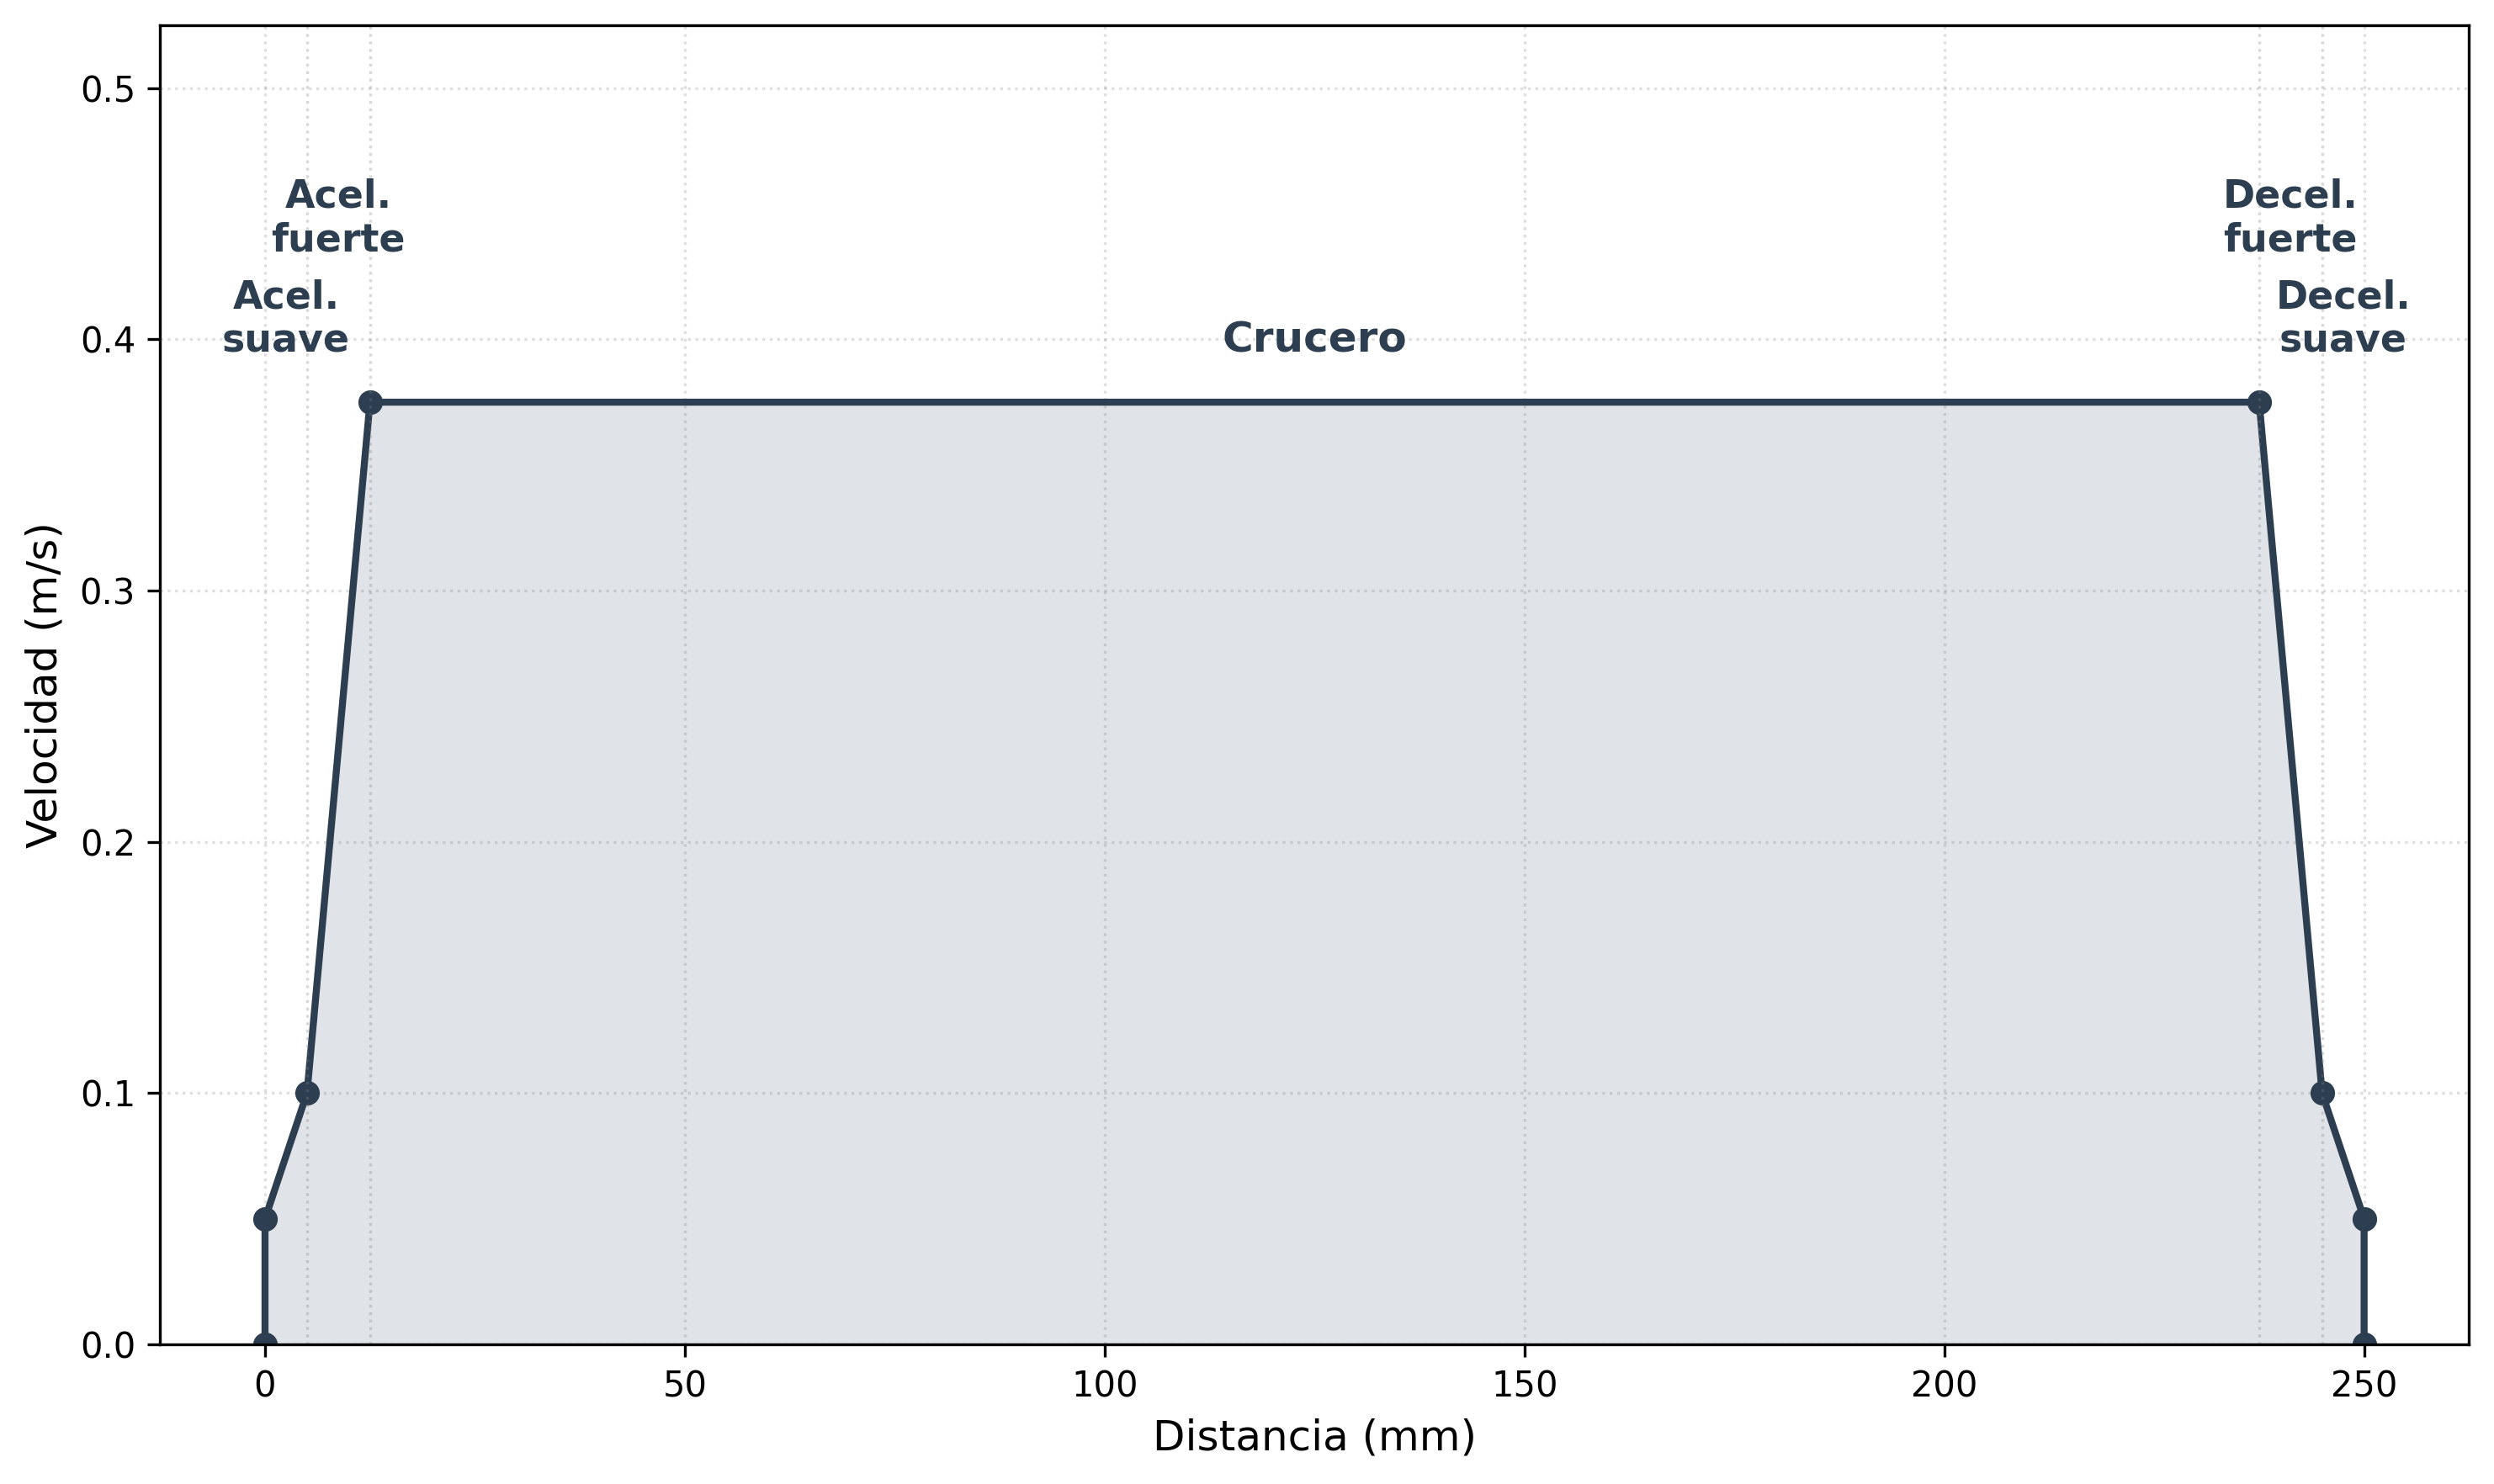
\includegraphics[width=0.8\textwidth]{imagenes/perfil_trapezoidal_velocidad.png}
    \caption{Perfil trapezoidal de velocidad con 5 zonas de transición}
    \label{fig:perfil_trapezoidal}
\end{figure}

\subsubsection{Cálculo Dinámico de Velocidad}

La velocidad en cada paso se calcula mediante interpolación lineal dentro de cada zona:

\begin{equation}
v(n) = v_{inicio} + \frac{(v_{fin} - v_{inicio}) \cdot (n - n_{inicio})}{n_{fin} - n_{inicio}}
\end{equation}

donde $n$ es el paso actual, $n_{inicio}$ y $n_{fin}$ delimitan la zona, y $v_{inicio}$, $v_{fin}$ son las velocidades en los extremos de la zona.

Este cálculo se ejecuta en cada paso dentro del loop principal (~10kHz), actualizando el registro OCR1A del Timer1 que controla la frecuencia de interrupción y, por ende, la frecuencia de pulsos STEP.

\subsubsection{Adaptación para Movimientos Cortos}

Movimientos muy cortos (<100 pasos, ~2.5mm) requieren tratamiento especial:

\begin{itemize}
    \item Velocidad crucero limitada a 2000 pasos/s (vs 10,000 pasos/s nominal)
    \item Zonas de aceleración/desaceleración reducidas a 25\% cada una
    \item Zona de crucero mínima (50\% restante)
\end{itemize}

Esta adaptación previene oscilaciones y garantiza precisión de posicionamiento incluso en movimientos de un solo paso.

\subsubsection{Sincronización Multi-Eje}

Para movimientos diagonales (ambos ejes simultáneos), el firmware implementa sincronización temporal para garantizar trayectorias rectilíneas (Figura \ref{fig:sincronizacion_multieje}).

\textbf{Algoritmo de sincronización}:

\begin{enumerate}
    \item Se calculan las distancias absolutas para cada eje: $d_H = |x_{target} - x_{actual}|$ y $d_V = |y_{target} - y_{actual}|$
    \item Se determina el eje dominante (mayor distancia a recorrer)
    \item El eje dominante utiliza su velocidad crucero nominal ($v_{cruise,H} = 15000$ pasos/s o $v_{cruise,V} = 12000$ pasos/s)
    \item El eje subordinado escala su velocidad proporcionalmente:
    \begin{equation}
    v_{sub} = v_{dom} \times \frac{d_{sub}}{d_{dom}}
    \end{equation}
    \item Se verifica que $v_{sub} \geq 500$ pasos/s (velocidad mínima). Si es menor, se recalcula invirtiendo roles.
    \item Ambos perfiles trapezoidales se inician simultáneamente con sus velocidades ajustadas
\end{enumerate}

\textbf{Resultado}: Ambos ejes completan su movimiento en el mismo tiempo total $T_{total}$, generando una trayectoria rectilínea en el plano XY. El error de linealidad es <1mm en trayectorias de 500mm.

\begin{figure}[H]
    \centering
    % TODO: Insertar diagrama de sincronización multi-eje
    % Mostrar: dos ejes con diferentes distancias, perfiles de velocidad escalados, trayectoria resultante
    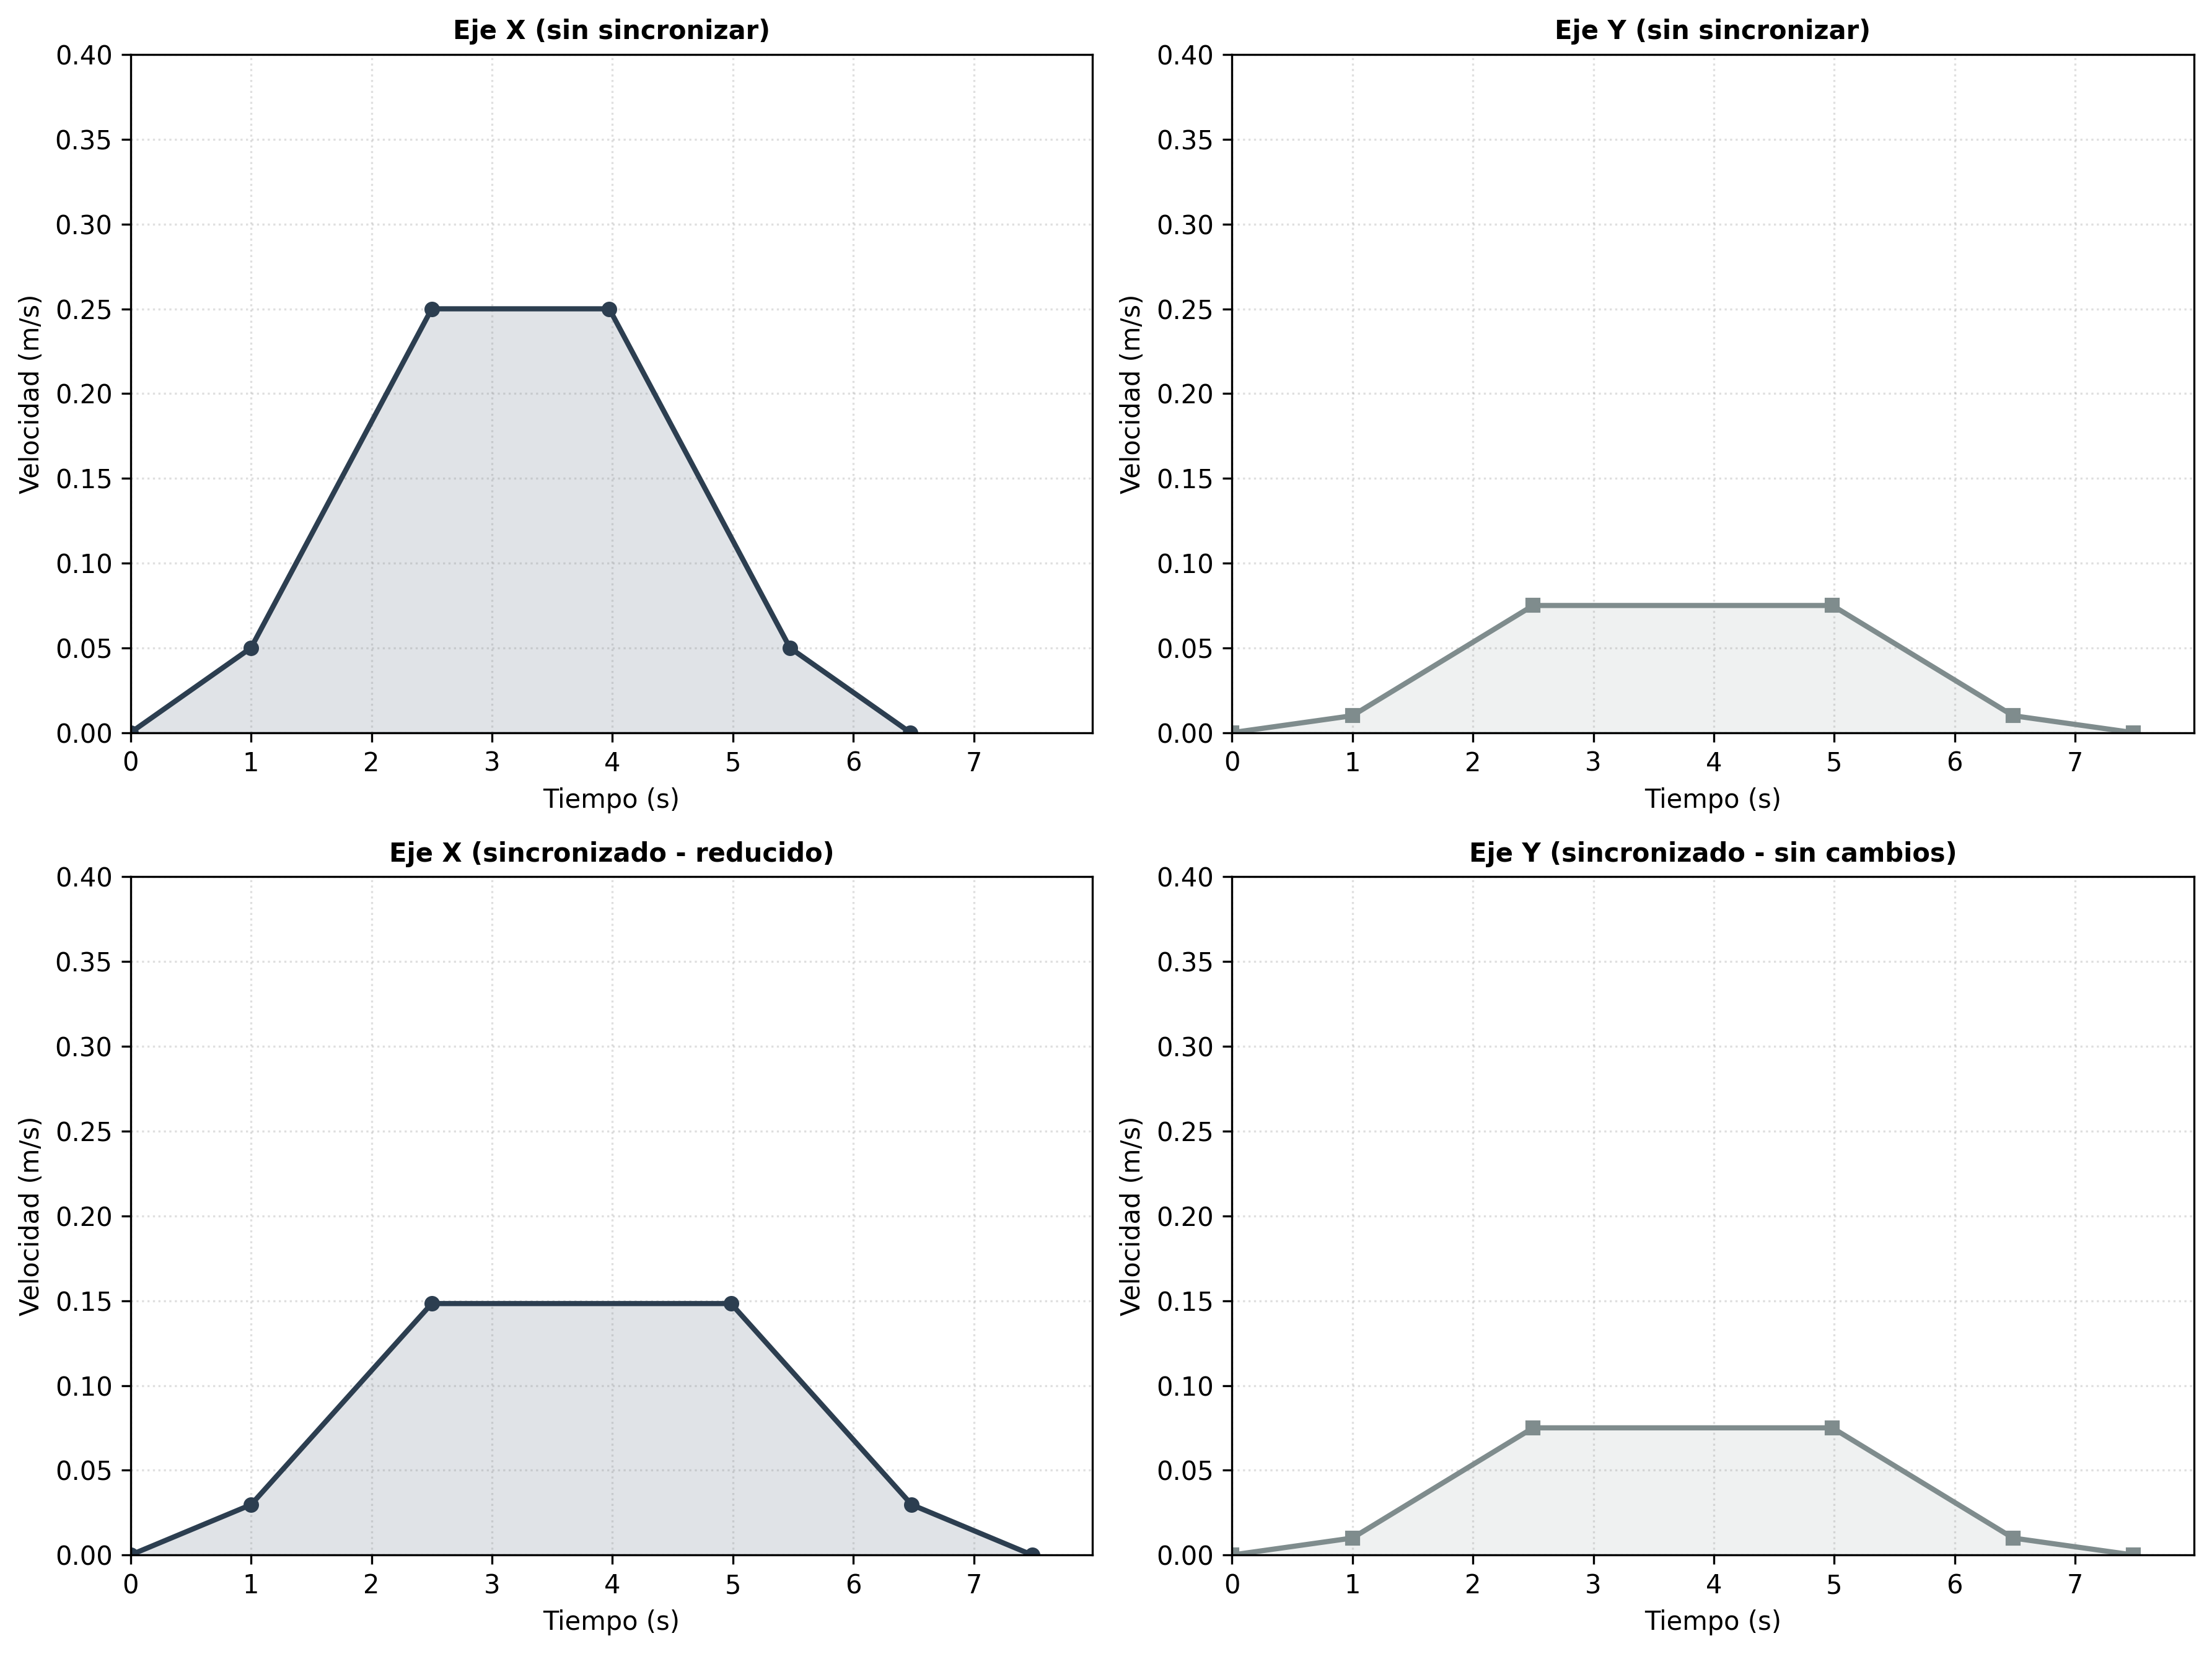
\includegraphics[width=0.9\textwidth]{imagenes/sincronizacion_multieje.png}
    \caption{Sincronización de perfiles de velocidad para movimientos diagonales}
    \label{fig:sincronizacion_multieje}
\end{figure}

\textbf{Ejemplo numérico}: Para un movimiento de $d_H = 4000$ pasos (100mm) y $d_V = 2000$ pasos (10mm):
\begin{itemize}
    \item Eje horizontal (dominante): $v_{cruise,H} = 15000$ pasos/s
    \item Eje vertical (subordinado): $v_{cruise,V} = 15000 \times \frac{2000}{4000} = 7500$ pasos/s
    \item Tiempo total sincronizado: $T \approx 0.35$ s (considerando aceleraciones)
\end{itemize}
